%!TEX root = vorlage.tex

\subsection{Markov Random Fields}\label{subsec:markov-random-fields}
\tikzstyle{pixel}=[draw,black,circle,minimum size=10pt,inner sep=0pt,fill=red!50]
\tikzstyle{label}=[draw,black,circle,minimum size=10pt,inner sep=0pt,fill=blue!50]
\tikzstyle{edge}=[very thick]
\begin{figure}
    \centering
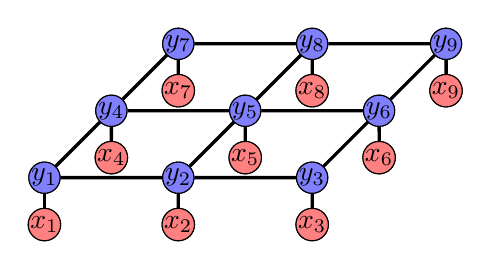
\begin{tikzpicture}[scale=1.7]
    \node (x1)[pixel] at (0.0,1.15) {$x_1$};
    \node (x2)[pixel] at (1.0,1.15) {$x_2$};
    \node (x3)[pixel] at (2.0,1.15) {$x_3$};
    \node (x4)[pixel] at (0.5,1.65) {$x_4$};
    \node (x5)[pixel] at (1.5,1.65) {$x_5$};
    \node (x6)[pixel] at (2.5,1.65) {$x_6$};
    \node (x7)[pixel] at (1.0,2.15) {$x_7$};
    \node (x8)[pixel] at (2.0,2.15) {$x_8$};
    \node (x9)[pixel] at (3.0,2.15) {$x_9$};

    \node (y1)[label] at (0.0,1.5) {$y_1$};
    \node (y2)[label] at (1.0,1.5) {$y_2$};
    \node (y3)[label] at (2.0,1.5) {$y_3$};
    \node (y4)[label] at (0.5,2.0) {$y_4$};
    \node (y5)[label] at (1.5,2.0) {$y_5$};
    \node (y6)[label] at (2.5,2.0) {$y_6$};
    \node (y7)[label] at (1.0,2.5) {$y_7$};
    \node (y8)[label] at (2.0,2.5) {$y_8$};
    \node (y9)[label] at (3.0,2.5) {$y_9$};

    \draw[edge] (y1) -- (y2);
    \draw[edge] (y1) -- (y4);
    \draw[edge] (y2) -- (y3);
    \draw[edge] (y2) -- (y5);
    \draw[edge] (y3) -- (y6);
    \draw[edge] (y4) -- (y5);
    \draw[edge] (y4) -- (y7);
    \draw[edge] (y5) -- (y6);
    \draw[edge] (y5) -- (y8);
    \draw[edge] (y6) -- (y9);
    \draw[edge] (y7) -- (y8);
    \draw[edge] (y8) -- (y9);

    \draw[edge] (x1) -- (y1);
    \draw[edge] (x2) -- (y2);
    \draw[edge] (x3) -- (y3);
    \draw[edge] (x4) -- (y4);
    \draw[edge] (x5) -- (y5);
    \draw[edge] (x6) -- (y6);
    \draw[edge] (x7) -- (y7);
    \draw[edge] (x8) -- (y8);
    \draw[edge] (x9) -- (y9);

    %\draw [dashed] (-0.5,-0.3) -- (2,-0.3) -- (3.5,1.5) -- (0.5,1.5) -- (-0.5,-0.3);
    \node (x1)[pixel] at (0.0,1.15) {$x_1$};
    \node (x2)[pixel] at (1.0,1.15) {$x_2$};
    \node (x3)[pixel] at (2.0,1.15) {$x_3$};
    \node (x4)[pixel] at (0.5,1.65) {$x_4$};
    \node (x5)[pixel] at (1.5,1.65) {$x_5$};
    \node (x6)[pixel] at (2.5,1.65) {$x_6$};
    \node (x7)[pixel] at (1.0,2.15) {$x_7$};
    \node (x8)[pixel] at (2.0,2.15) {$x_8$};
    \node (x9)[pixel] at (3.0,2.15) {$x_9$};

    \node (y1)[label] at (0.0,1.5) {$y_1$};
    \node (y2)[label] at (1.0,1.5) {$y_2$};
    \node (y3)[label] at (2.0,1.5) {$y_3$};
    \node (y4)[label] at (0.5,2.0) {$y_4$};
    \node (y5)[label] at (1.5,2.0) {$y_5$};
    \node (y6)[label] at (2.5,2.0) {$y_6$};
    \node (y7)[label] at (1.0,2.5) {$y_7$};
    \node (y8)[label] at (2.0,2.5) {$y_8$};
    \node (y9)[label] at (3.0,2.5) {$y_9$};
\end{tikzpicture}
\caption{\gls{CRF} with 4-neighborhood. Each node $x_i$ represents a pixel and
         each node $y_i$ represents a label.}
\label{fig:crf-image}
\end{figure}
\Glspl{MRF} are undirected probabilistic graphical models which are wide-spread
model in computer vision. The overall idea of \glspl{MRF} is to assign a random
variable for each feature and a random variable for each pixel which gets
labeled as shown in~\cref{fig:crf-image}. For example, a \gls{MRF} which is
trained on images of the size
$\SI{224}{\pixel} \times \SI{224}{pixel}$ and gets the raw RGB values as
features has
\[\underbrace{224 \cdot 224 \cdot 3}_{\text{input}} + \underbrace{224 \cdot 224}_{\text{output}} = \num{200704}\]
random variables. Those random variables are conditionally independent, given
their local neighborhood. These (in)dependencies can be expressed with a graph.

Let $G=(\mathcal{V}, \mathcal{E})$ be the associated undirected graph of an
\gls{MRF} and $\mathcal{C}$ be the set of all maximal cliques in that graph.
Nodes represent random variables $\mathbf{x}, \mathbf{y}$ and edges represent
conditional dependencies. Just like in
\crefname{subsec:graph-based-image-segmentation}, the
4-neighborhood~\cite{shotton2006textonboost} and the 8-neighborhood are
reasonable choices for constructing the graph.

Typically, random variables $\mathbf{y}$ represent the class of a single pixel,
random variables $\mathbf{x}$ represent a pixel values and edges represent
pixel neighborhood in computer vision problems segmentation problems where
\glspl{MRF} are used. Accordingly, the random variables $\mathbf{y}$ live on
$1, \dots, \text{nr of classes}$ and the random variables $\mathbf{x}$
typically live on $0, \dots, 255$ or $[0, 1]$.

The probability of $\mathbf{x}, \mathbf{y}$ can be expressed as
\[P(\mathbf{x}, \mathbf{y}) = \frac{1}{Z} e^{-E(\mathbf{x}, \mathbf{y})}\]
where $Z = \sum_{\mathbf{x}, \mathbf{y}} e^{-E(\mathbf{x}, \mathbf{y})}$ is a normalization term called
the \textit{partition function} and $E$ is called the \textit{energy function}.
A common choice for the energy function is
\[E(\mathbf{x}, \mathbf{y}) = \sum_{c \in \mathcal{C}} \psi_c(\mathbf{x}, \mathbf{y})\]
where $\psi$ is called a \textit{clique potential}. One choice for cliques
of size two $\mathbf{x}, \mathbf{y} = (x_1, x_2)$ is~\cite{kato2006markov}
\[\psi_c(x_1, x_2) = w \delta(x_1, x_2) = \begin{cases}+w &\text{if } x_1 \neq x_2\\-w &\text{if } x_1 = x_2\end{cases}\]

According to~\cite{murphy2012machine}, the most common way of inference over
the posterior \gls{MRF} in computer vision problems is \gls{MAP} estimation.


Detailed introductions to \glspl{MRF} are given by
\cite{blake2011markov,murphy2012machine}. \glspl{MRF} are used by \cite{zhang2001segmentation} and \cite{moser2012markov}
for image segmentation.

% Characterizations of MRF:
% Label space: binary vs multi-label; homogeneous vs heterogeneous
% Order: unary vs pairwise vs higher-order
% Structure: chain vs tree vs grid vs general graph; neighborhood size
% Potentials: submodular, convex, compressible

% Markov Random Fields for Computer Vision (Part 1)
% http://users.cecs.anu.edu.au/~sgould/papers/part1-MLSS-2011.pdf  --- very nice!
% http://users.cecs.anu.edu.au/~sgould/papers/part2-MLSS-2011.pdf
% http://users.cecs.anu.edu.au/~sgould/papers/part3-MLSS-2011.pdf

% Markov Random Field Image Models and Their Applications to Computer Vision
% http://www.mathunion.org/ICM/ICM1986.2/Main/icm1986.2.1496.1517.ocr.pdf


\subsection{Conditional Random Fields}\label{subsec:conditional-random-fields}

\Glspl{CRF} are \glspl{MRF} where all clique potentials are conditioned on
input features~\cite{murphy2012machine}. This means, instead of learning the
distribution $P(\mathbf{y}, \mathbf{x})$, the task is reformulated to learn the
distribution $P(\mathbf{y}| \mathbf{x})$. One consequence of this reformulation
is that \glspl{CRF} need much less parameters as the distribution of
$\mathbf{x}$ does not have to be estimated. Another advantage of \glspl{CRF}
compared to \glspl{MRF} is that no distribution assumption about $\mathbf{x}$
has to be made.

A \gls{CRF} has the partition function $Z$:
\[Z(\mathbf{x}) = \sum_{\mathbf{y}} P(\mathbf{x}, \mathbf{y})\]

and joint probability distribution

\[P(\mathbf{y} | \mathbf{x}) = \frac{1}{Z(\mathbf{x})} \prod_{c \in \mathcal{C}} \psi_c(\mathbf{y}_c | \mathbf{x})\]

The simplest way to define the clique potentials $\psi$ is the count of the
class $\mathbf{y}_c$ given $\mathbf{x}$ added with a positive smoothing
constant to prevent the complete term from getting zero.

\Glspl{CRF} as described in~\cite{associative09} have reached top performance
in PASCAL VOC 2010~\cite{VOC2010Results} and are also used in
\cite{multiscale04,shotton2006textonboost} for semantic segmentation.

A method similar to \glspl{CRF} was proposed in~\cite{gonfaus2010harmony}.
The system of Gonfaus~et.al. ranked~\nth{1} by mean accuracy in the segmentation
task of the PASCAL VOC 2010 challenge~\cite{everingham2010pascal}.

An introduction to \glspl{CRF} is given by~\cite{sutton2011introduction}.
